\documentclass[11pt]{article}
\usepackage[portuguese]{babel}
\usepackage[utf8]{inputenc}
\usepackage[T1]{fontenc}
\usepackage{textcomp}
\usepackage{lmodern}
\usepackage{graphicx}

\setlength{\parskip}{2ex}
\def\aspa{\textquotesingle}

\setlength{\pdfpagewidth}{210truemm}
\setlength{\pdfpageheight}{297truemm}
\pdfadjustspacing=1

\topmargin -0.6in
\textheight 250truemm

\title{\vspace{8em} \huge{Wiki UFC} \\ \vspace{0.1em} \small{Estudo de Viabilidade}}
\author{
        \vspace{5em} \\
        \small{Adriano Tavares} \\
        \small{Álinson Santos}  \\
        \small{André Castro}    \\
        \small{Luís Henrique}   \\
        \small{Rafael Barbosa}
}
\date{\today}

\begin{document}

\maketitle
\pagebreak

\tableofcontents
\pagebreak

% ===================
% Título da Aplicação
% ===================
\section{Título da Aplicação}

Wiki UFC

% ======================
% Descrição da Aplicação
% ======================
\section{Descrição da Aplicação}

Sistema online colaborativo onde os alunos poderão compartilhar informações sobre
as disciplinas que estão cursando. Cada disciplina terá um espaço próprio, contendo
um Wiki (para receber notas de aulas), mural de mensagens (para os alunos serem
notificados sobre algum evento), calendário (contendo datas de provas, trabalhos, etc)
e um repositório de arquivos (contendo provas passadas, listas de exercícios, etc).


% =====================
% Objetivo da Aplicação
% =====================

\section{Objetivo da Aplicação}

Permitir que os alunos tenham acesso rápido e organizado a todo o material
disponibilizado pelos professores durante as aulas (incluindo listas de exercícios e
notas de aulas), e que se mantenham atualizados sobre quaisquer eventos da
disciplina.


% =============
% Justificativa
% =============

\section{Justificativa}

Atualmente, não há um local próprio para os alunos lerem e publicarem informações
sobre as disciplinas que estão cursando. Como conseqüência, muitos meios diferentes
são utilizados, como listas de emails, páginas web, ou, na maioria dos casos, o diálogo
boca-a-boca. O problema dessa abordagem é que, para o aluno, é muito difícil se
manter atualizado. Ele precisa acompanhar, constantemente, cada um desses meios,
ou corre o risco de perder alguma mensagem.
Para o material disponibilizado pelo professor, o problema é ainda maior: para
conseguir as notas de aula ou listas de exercícios de uma disciplina, geralmente o
aluno precisa tomar emprestado o material de um colega e pagar por fotocópias de
baixa qualidade, que serão descartadas ao término do semestre. Para conseguir
material de semestres passados, então, o processo é ainda mais complexo, se não
impossível, na maioria dos casos.
% ================
% Solução Proposta
% ================


\section{Solução Proposta}

O desenvolvimento de um sistema online onde os alunos possam ler e publicar
informações livremente, utilizando Ruby on Rails, um framework para
desenvolvimento Web na linguagem de programação interpretada Ruby.

% =====================
% Delimitação do Escopo
% ====================


\section{Delimitação do Escopo}

\subsection{O que será feito?}

Estão previstos quatro módulos principais

\begin{description}
	\item[Wiki] Uma área textual livre editável por qualquer usuário do sistema, para conter as notas de aula de cada disciplina;
	\item[Mural] Uma área para postagem de notícias sobre as disciplinas;
	\item[Calendário] Para receber datas de provas e entregas de trabalhos;
	\item[Repositório] Uma área para receber arquivos adicionais, tais como listas de exercícios e provas passadas.
\end{description}

\subsection{O que não será feito?}

Sendo um sistema voltado para o aluno, e não para o professor, não há planos sobre
implementar sistemas de entrega de trabalhos, aulas e avaliações online em tempo
real, nem qualquer recurso semelhante encontrado em outros softwares de e-learning.
% ==================
% Produtos Esperados
% ==================


\section{ Benefícios Esperados}

Entre os principais benefícios esperados estão:

\begin{description}
	\item[Centralização]
     As informações sobre todas as disciplinas estarão juntas em um local, então, para os alunos, será
     mais fácil verificar em quais delas há novidades.
	\item[Atualização]
     Como qualquer aluno poderá publicar informações, é provável que o conteúdo esteja sempre bem
     atualizado. Qualquer desatualização poderá ser rapidamente corrigida.
	\item[Descentralização]
     Para os alunos, o processo de publicação será descentralizado: ninguém será unicamente
     responsável por manter o conteúdo no ar.
\end{description}
% ========
% Produtos
% ========


\section{Produtos}

\subsection{Produtos Intermediários}

A documentação completa do sistema, ou seja:
\begin{itemize}
	\item Diagrama de barras e rede de atividades
	\item Estudo de viabilidade
	\item Especificação de requisitos
	\item Projeto da aplicação
\end{itemize}

\subsection{Produto Final}

O sistema anteriormente descrito, com código-fonte e executável.


% ============
% Público Alvo
% ============

\section{Público Alvo}
O público alvo, a priori, são os alunos do curso de graduação do curso de Computação,
UFC. Posteriormente, este este público pode ser expandido para englobar tanto os
alunos de pós-graduação, quanto os alunos de outros cursos da UFC.

% ==========
% Restrições
% ==========


\section{Restrições}
As restrições podem ser divididas em dois grupos:

\subsection{Restrições de Projeto}

\begin{description}
	\item[Prazo] A entrega do sistema deve ser efetuada até o dia 26 de junho de 2007.
	\item[Marcos] Alguns marcos pré-estabelecidos pelo cliente devem ser seguidos.
	\item[Equipe] A equipe será composta por no máximo cinco pessoas
	\item[Público Alvo] O sistema será focado para atender as necessidades dos alunos.
\end{description}

\subsection{Restrições Técnicas}

\begin{description}
	\item[Linguagem] A priori, a aplicação poderia apenas ser desenvolvida utilizando as linguagens Java ou PHP. Porém, foi negociado com o cliente o desenvolvimento utilizando a linguagem Ruby.
	\item[Requisitos da Aplicação] O usuário necessitará de um browser recente com conexão à Internet.
\end{description}

% ============
% Alternativas
% ============


\section{Alternativas}

Como alternativa a algumas restrições e recursos requeridos temos:

\begin{itemize}   
	\item A negociação com cliente permitiu o desenvolvimento do sistema utilizando outra linguagem de programação, Ruby.
	\item Os programadores utilizarão seus computadores pessoais, da universidade ou de LAN houses para fins de desenvolvimento.
\end{itemize}

% ===================
% Recursos Requeridos
% ===================


\section{Recursos Requeridos}

A aplicação será desenvolvida em plataforma web, utilizando o framework Ruby on
Rails. Os desenvolvedores necessitarão de computadores conectados a Internet para
desenvolvimento e upload/download das versões do sistema. Para os usuários, o único
software necessário será um browser recente, com conexão à Internet. Do lado do
servidor, a aplicação executará em um servidor web com suporte a Ruby, e em um
banco de dados qualquer.
Quanto aos recursos humanos, a equipe dispõe de cinco integrantes, sendo todos
desenvolvedores e um também gerente de projeto.

% ======
% Riscos
% ======


\section{Riscos}

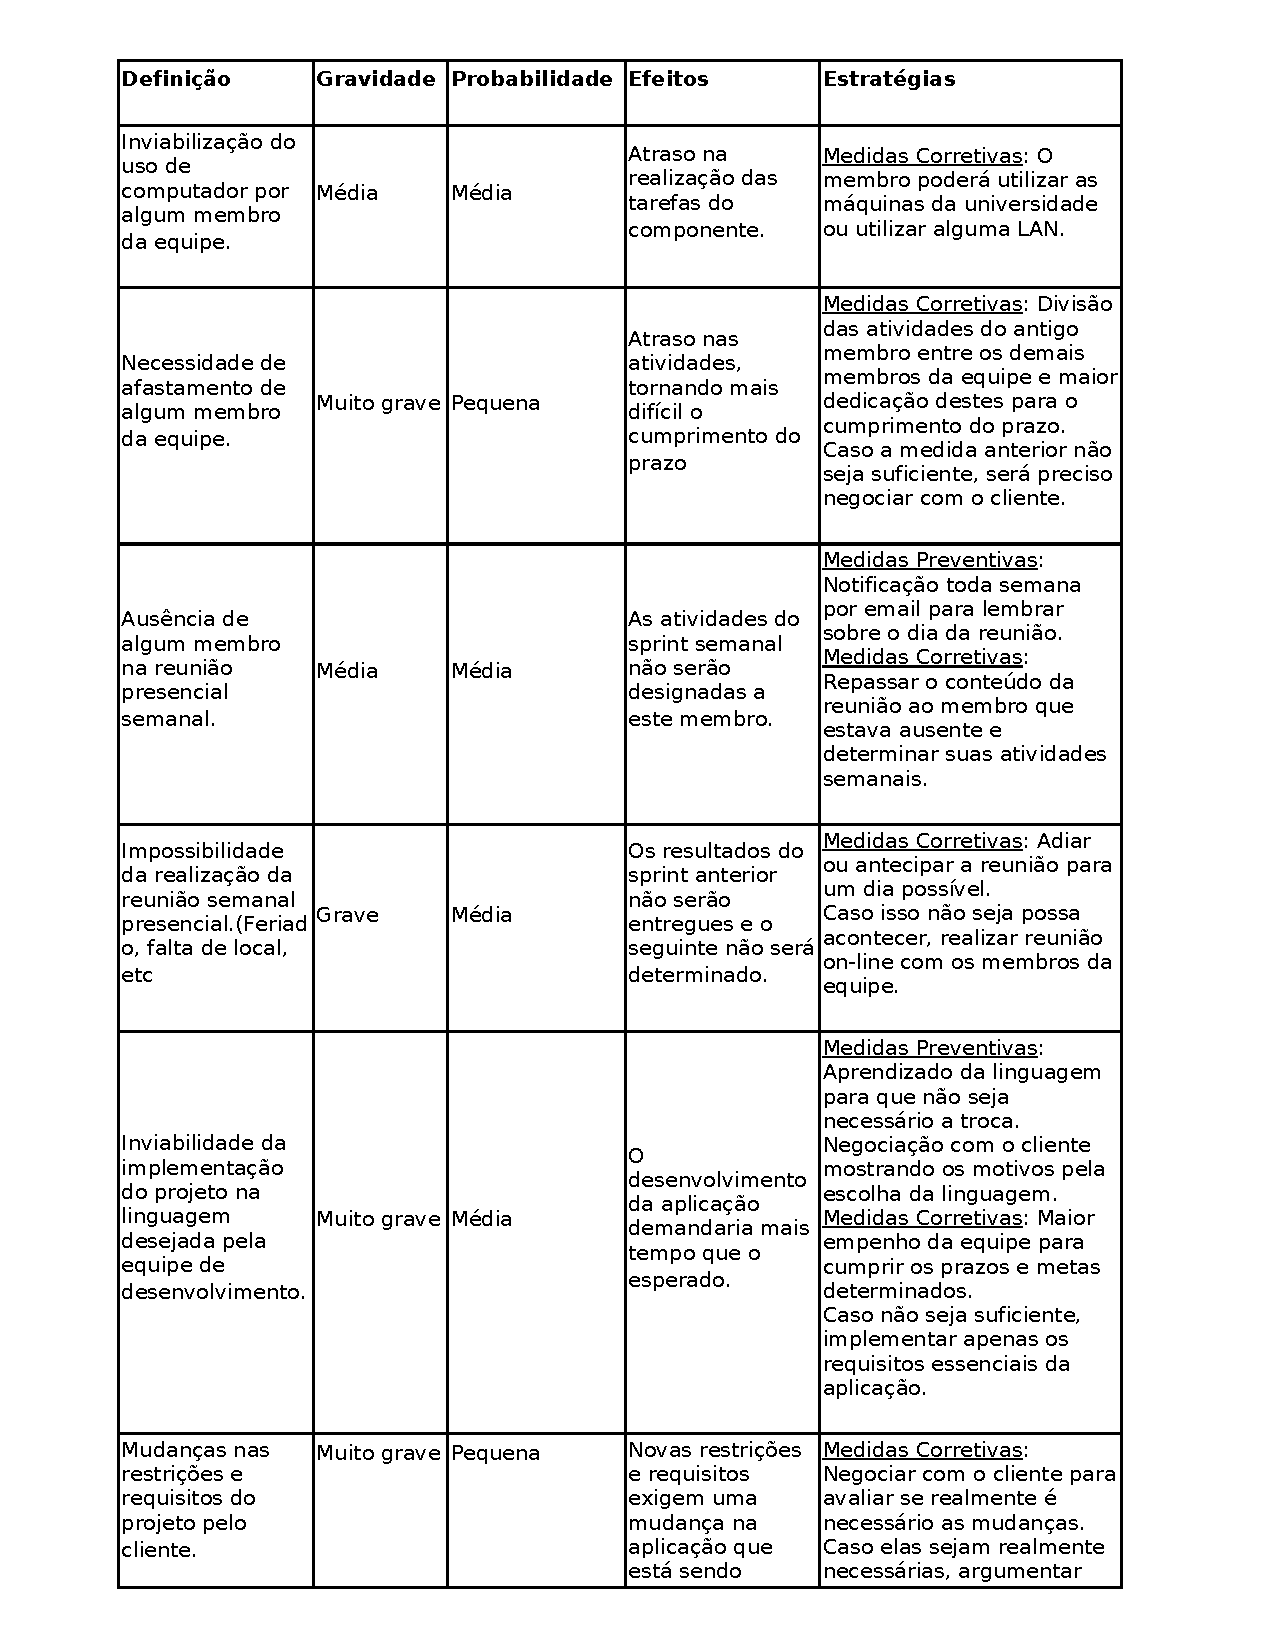
\includegraphics[width=1.30\textwidth]{riscos.pdf}\\

% ==================
% Modelo de Processo
% ==================


\section{Modelo de Processo}

Para o desenvolvimento, será adotado a metodologia ágil Scrum.

\begin{itemize}
	\item Um backlog será criado para manter a lista de tarefas pendentes do projeto;
	\item Semanalmente, haverá uma reunião, na qual a equipe escolherá alguns itens do backlog para implementar durante o sprint;
	\item Ao final de cada sprint, uma nova reunião será feita, onde cada participante irá apresentar trabalho que desenvolveu ao longo da semana.
\end{itemize}

\end{document}

